\documentclass[aspectratio=169]{beamer}

\usepackage[utf8]{inputenc}
\usepackage[ngerman]{babel}
\usepackage{minted}
\usepackage{hyperref}
\usepackage{color}
\usepackage{tikz}
\usepackage{amsmath}
\usetikzlibrary{arrows}
\usetikzlibrary{decorations.pathreplacing}

\usemintedstyle{emacs}

\usetheme[progressbar=head,block=fill]{metropolis}

\title{Final Talk LiL4}
\subtitle{Group3 - speedDreams}
\date{July 11, 2017}
\author{Alexander Reisner \and
Alexander Weidinger \and
David Werner}
\institute{Technische Universität München}
\begin{document}
  \renewcommand{\figurename}{\tiny Fig.}
  \maketitle

  \begin{frame}{ToC}
    \tableofcontents
  \end{frame}

  \section{Introduction}
  \subsection{Overview}
  \begin{frame}{Project Overview}
    [ Complete Graphic of the Project ]
  \end{frame}

  \subsection{Trask Description}
  \begin{frame}{Our Task}
    [ List of our points in the specification book ]
  \end{frame}

  \subsection{Sub Projects}
  \begin{frame}{Task allocation}
    \begin{itemize}
      \item Alexander Weidinger
      \begin{itemize}
        \item Extend SpeedDreams 2 (SD2) by a virtual proximity sensor
        \item Build data exchange between SD2 and Simulation Coupler (SimCoupler)
        \item Create data exchange between SimCoupler and QEMU S/A VM
      \end{itemize}
      \item Alexander Reisner
      \begin{itemize}
        \item Introduce the QEMU S/A VM
        \item Exchange data between SimCoupler and QEMU S/A VM
        \item Implement mosquitto client to forward data to the ECUs
      \end{itemize}
      \item David Werner
      \begin{itemize}
        \item Implement an autonomous parking algorithm
        \item Implement mosquitto client to forward calculated control data
      \end{itemize}
    \end{itemize}
  \end{frame}

  \section{Alexander Weidinger}
  \subsection{Proximity Sensor}
  \begin{frame}{Related Work}
    \begin{itemize}
      \item<1-> Research Phase: Find implementations of such sensor for TORCS / SD2
      \item<2-> Adapt the found sensor implementation for usage in SD2 and test it
      \item<3-> Resignation: The sensor isn't appropriate for our use case
      \item<4-> \textbf{Write our own proximity sensor}
    \end{itemize}
  \end{frame}

  \subsection{Implementation Comparison}
  \begin{frame}{Comparison of Implementations}
    \begin{columns}
      \begin{column}{0.5\textwidth}
        \begin{figure}
        \begin{tikzpicture}[scale=0.75]
          % car 1
          \draw (0,0) -- (2,0) -- (2,3) -- (0,3) -- (0,0);
          \fill (1, 1.5) circle [radius=0.05];
          % car 2
          \draw (3,1) -- (5,1) -- (5,4) -- (3,4) -- (3,1);
          \fill (4, 2.5) circle [radius=0.05];
          % line between the two midpoints
          \draw (1, 1.5) -- (4, 2.5);
          % sensor lines
          \foreach \x in {0, 30, ..., 330}
          {
          \draw[red, dashed] (1, 1.5) -- +(\x : 3);
          }
          % distance bracket
          \draw[decoration={brace,mirror,raise=5pt},decorate] (1, 1.5) -- (4, 2.5) node[black,midway,yshift=-0.5cm] {\footnotesize $d_1$};
        \end{tikzpicture}
        \caption{\tiny Proximity sensors implemented by the Simulated Car Racing Championship 2015}
      \end{figure}
      \end{column}
      \begin{column}{0.5\textwidth}
        \begin{figure}
        \begin{tikzpicture}[scale=0.75]
          % car 1
          \draw (0,0) -- (2,0) -- (2,3) -- (0,3) -- (0,0);
          \fill (1, 1.5) circle [radius=0.05];
          % car 2
          \draw (3,1) -- (5,1) -- (5,4) -- (3,4) -- (3,1);
          \fill (4, 2.5) circle [radius=0.05];
          % sensor
          \draw[blue, dashed] (2, 1.5) -- +(0 : 4); % line
          \fill[blue] (2, 1.5) circle [radius=0.05]; % starting point
          % intersections
          \draw[blue] (3, 1.5) circle [radius=0.1];
          \draw[blue]  (5, 1.5) circle [radius=0.1];
          % distance bracket
          \draw[decoration={brace,mirror,raise=5pt},decorate] (2, 1.5) -- (3, 1.5) node[black,midway,yshift=-0.5cm] {\footnotesize $d_2$};
        \end{tikzpicture}
        \caption{\tiny (Laser) proximity sensors implemented by us}
      \end{figure}
      \end{column}
    \end{columns}
  \end{frame}

  \section{Alexander Reisner}

  \subsection{Mosquitto}
  \begin{frame}{Mosquitto}
        \begin{figure}
        \begin{tikzpicture}[scale=0.75]
          % server
          \draw (5,1) -- (7,1) -- (7,4) -- (5,4) -- (5,1);
          \fill (6, 2.5) circle [radius=0.05] node[yshift=0.5cm] {\footnotesize $Server$};
          %subscriber
          \draw (10,0) -- (12,0) -- (12,3) -- (10,3) -- (10,0);
          \fill (11, 1.5) circle [radius=0.05] node[yshift=0.5cm] {\footnotesize $Subsciber$};
          % line between server and subscriber
          \draw [-triangle 60] (11, 1.5) -- (6, 2.5) node[black,midway,yshift=-0.5cm] {\footnotesize $subscibe$};
        \end{tikzpicture}
        \caption{\tiny Subscriber}
      \end{figure}
  \end{frame}

  \begin{frame}{Mosquitto}
        \begin{figure}
        \begin{tikzpicture}[scale=0.75]
          % publisher
          \draw (0,0) -- (2,0) -- (2,3) -- (0,3) -- (0,0);
          \fill (1, 1.5) circle [radius=0.05] node[yshift=0.5cm] {\footnotesize $Publisher$};
          % server
          \draw (5,1) -- (7,1) -- (7,4) -- (5,4) -- (5,1);
          \fill (6, 2.5) circle [radius=0.05] node[yshift=0.5cm] {\footnotesize $Server$};
          %subscriber
          \draw (10,0) -- (12,0) -- (12,3) -- (10,3) -- (10,0);
          \fill (11, 1.5) circle [radius=0.05] node[yshift=0.5cm] {\footnotesize $Subscriber$};
          % line between publisher and server
          \draw [-triangle 60] (1, 1.5) -- (6, 2.5) node[black,midway,yshift=-0.5cm] {\footnotesize $publish$};
          % line between server and subscriber
          \draw [-triangle 60] (6, 2.5) -- (11, 1.5) node[black,midway,yshift=-0.5cm] {\footnotesize $on\_message$};
        \end{tikzpicture}
        \caption{\tiny Publisher}
      \end{figure}
  \end{frame}


  \section{David Werner}
  
  \subsection{Autonomous Parking}
  \begin{frame}{Problem}
  	\begin{figure} [ht]
  		\centering
  		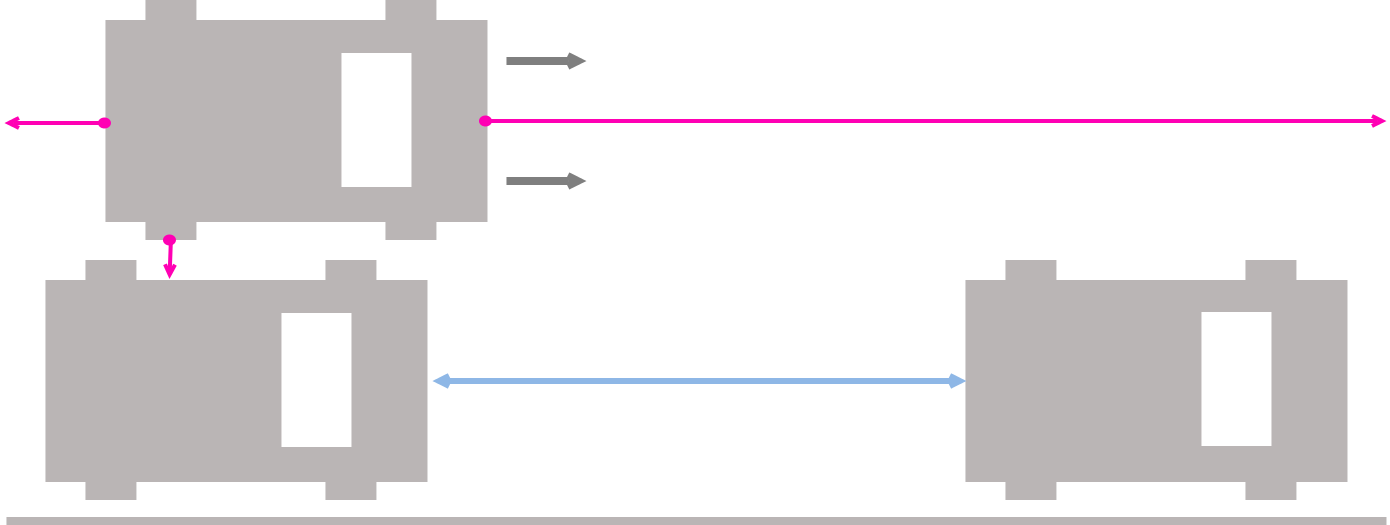
\includegraphics[width=0.8\textwidth]{david_images/Problem.png}
  		\caption{\tiny Car needs to autonomously pass by the parking lot, detect it and perform a parallel parking maneuver}
	\end{figure}
  \end{frame}
  
  \subsection{Algorithm}
  \begin{frame}{Basics}
  	\begin{itemize}
  	\item<1-> calculation of actuator data
  		\begin{itemize}
  		 \item<2-> velocity v
  		 \item<3-> steering angle $\phi$
  		\end{itemize}
  	\item<4-> no computation of an exact path
  	\item<5-> actuator data is determined by the evaluation of our 3-phase algorithm
  	\end{itemize}
  \end{frame}
   
  \begin{frame}{Phase 1 - Searching phase (1)}
  	\begin{figure} [ht]
  		\centering
  		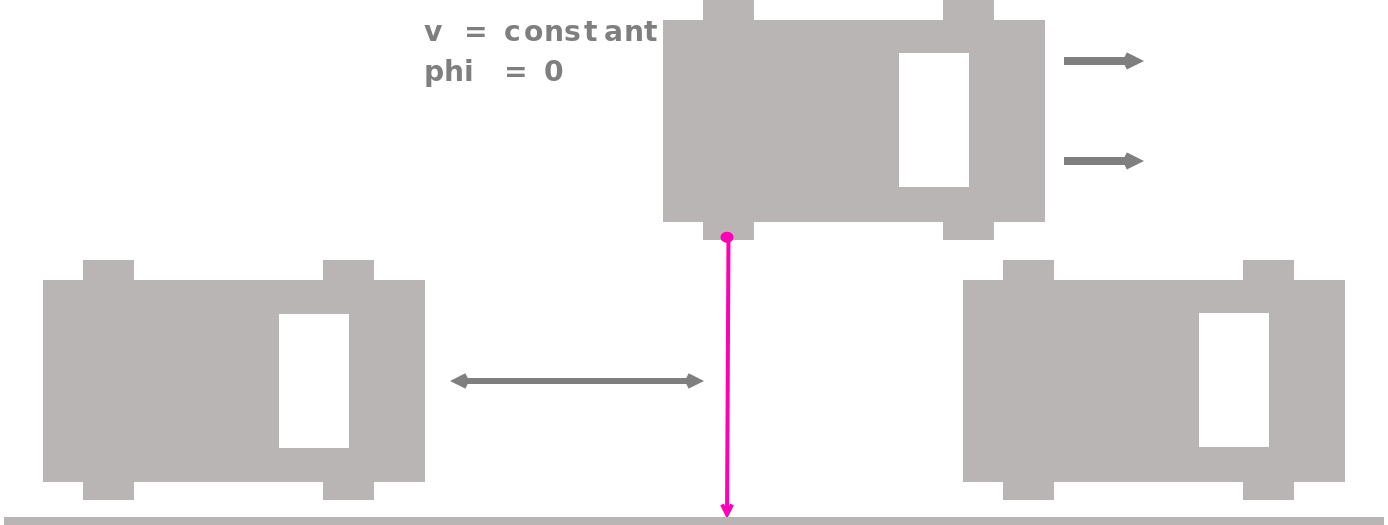
\includegraphics[width=1.0\textwidth]{david_images/FindLot1.png}
  		\caption{\tiny Car passes the potential parking lot and calculates its size}
	\end{figure}
  \end{frame}
  
  \begin{frame}{Phase 1 - Searching phase (2)}
  	\begin{figure} [ht]
  		\centering
  		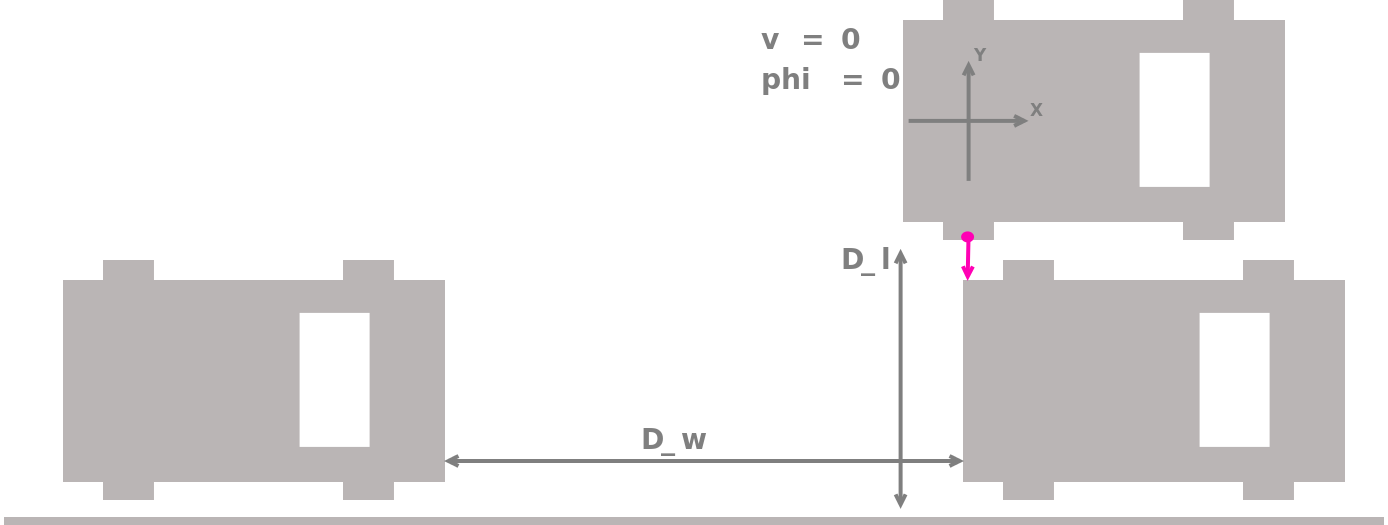
\includegraphics[width=0.9\textwidth]{david_images/FindLot2.png}
  		\caption{\tiny Algorithm creates environment and position information}
	\end{figure}
  \end{frame}
  
  \begin{frame}{Phase 2 - Calculation phase (1)}
    	\begin{itemize}
  		\item<1-> equations of vehicle's motion:
  			\begin{itemize}
  				\item<2-> $\dot{x} = v * cos(\phi) * cos(\theta)$
  				\item<3-> $\dot{y} = v * cos(\phi) * sin(\theta)$ 
  				\item<4-> $\dot{\theta} = \frac{v}{L} * sin(\phi)$ 
  			\end{itemize}
  		\item<5-> time dependant formulas for v and $\phi$ needed
  			\begin{itemize}
  				\item<6-> $\phi(t)$ - steering angle (based on max $\phi$)
  				\item<7-> $v(t)$ - velocity (based on max v)
  			\end{itemize}
  		\item<8-> time for whole menauever is estimated and optimized
  	\end{itemize}
  \end{frame}
  
  \begin{frame}{Phase 2 - Calculation phase (2)}
  	\begin{figure} [ht]
  		\centering
  		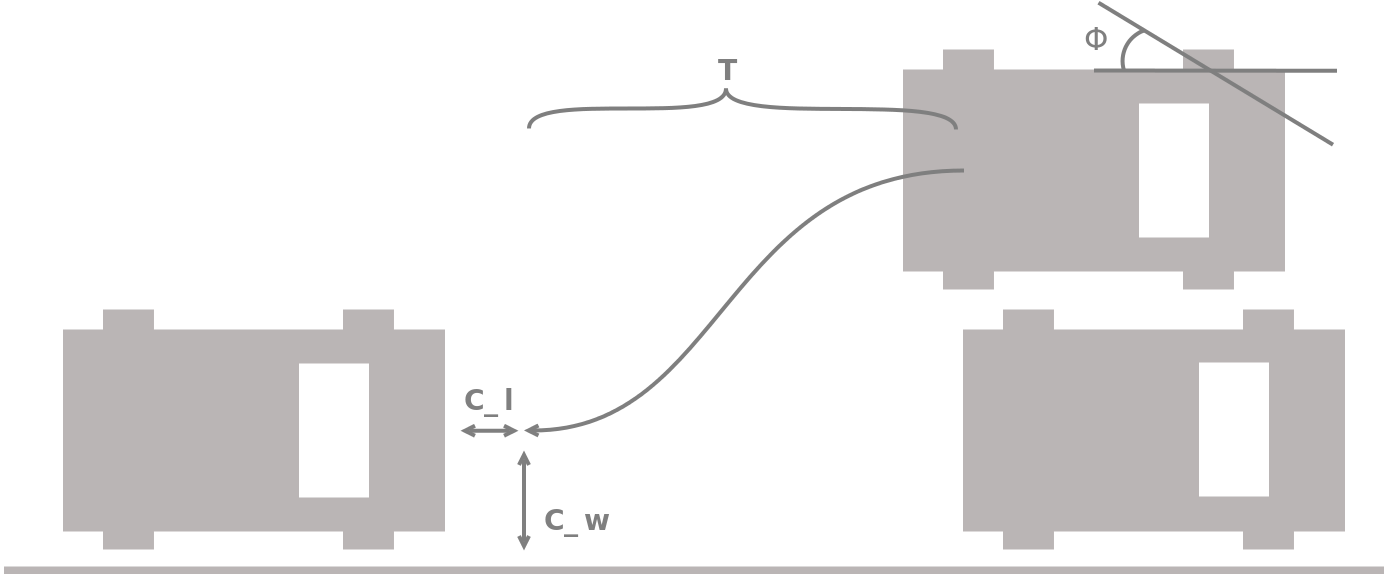
\includegraphics[width=0.9\textwidth]{david_images/Calculating.png}
  		\caption{\tiny Algorithm simulates parking maneuver to calculate duration and steering angle}
	\end{figure}
  \end{frame}
  
  \begin{frame}{Phase 3 - Parking phase}
  	\begin{figure} [ht]
  		\centering
  		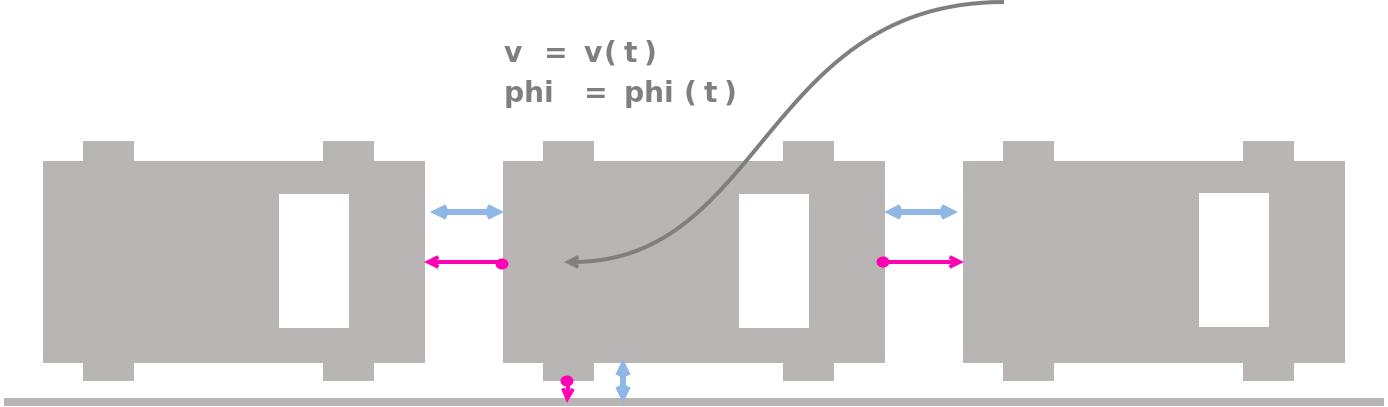
\includegraphics[width=0.9\textwidth]{david_images/Parked.png}
  		\caption{\tiny Algorithm steers and accelerates the car according to calculation until parking position is reached}
	\end{figure}
  \end{frame}
  
  \subsection{Problems and Limitations}
  \begin{frame}{Problems and Limitations}
  	\begin{itemize}
  		\item<1-> calculation of parking duration is based on magic number
  		\item<2-> longitudinal and lateral distance conditions seem to work not properly
  		\item<3-> safety distance needs to be higher than necessary
  	\end{itemize}
  \end{frame}
  \end{document}
